\documentclass[conference]{IEEEtran}

\usepackage[T1]{fontenc}
\usepackage{amsmath,amssymb,amsfonts}
\usepackage{graphicx}
\usepackage{booktabs}
\usepackage{array}
\usepackage{cite}
\usepackage{url}
\usepackage{microtype}
\usepackage{flushend}

% Keep small, positive gaps around floats and captions in the two-column layout.
\setlength{\textfloatsep}{8pt plus 2pt minus 2pt}
\setlength{\floatsep}{6pt plus 2pt minus 1pt}
\setlength{\intextsep}{8pt plus 2pt minus 2pt}
\setlength{\abovecaptionskip}{4pt}

\graphicspath{{figs/}}

\begin{document}

\title{Coronary Artery Disease Bayesian Classification:\
Derivation, Implementation, and Empirical Validation on the UCI Cleveland Dataset}

\author{}

\maketitle

\begin{abstract}
This study evaluates a mixed-type Naive Bayes classifier on the UCI Cleveland heart-disease dataset, with attention to outcome coding and the joint treatment of measurements and symptom categories. The documented processed Cleveland file was used, and a duplicate check confirmed that all 303 records could be retained. Four continuous variables were modeled with Gaussian likelihoods; chest-pain type and exercise-induced angina were modeled with Laplace-smoothed categorical likelihoods. The cohort includes 164 controls and 139 CAD-positive cases. Evaluation used a stratified 80/20 holdout, 1{,}000 bootstrap resamples, and $10 \times 5$-fold cross-validation. Across the 50 folds, adding symptom variables raised mean ROC-AUC from $0.732\pm0.052$ to $0.831\pm0.045$, a difference of $0.099$. Mixed NB and $\ell_2$-regularized logistic regression had similar AUCs ($0.831\pm0.045$ and $0.830\pm0.049$; exploratory paired-fold Wilcoxon $p=0.652$). On the holdout set, Mixed NB classified $80.3\%$ of cases correctly [95\% CI: $70.5\%$--$90.2\%$], with $82.1\%$ recall and AUC $0.891$ [95\% CI: $0.803$--$0.960$]. Some continuous variables departed from the Gaussian assumption, and age and maximum heart rate were correlated among controls ($r=-0.523$). Discrimination was comparable to logistic regression, but Mixed NB probabilities were less well calibrated (Brier score $0.183$ versus $0.168$). These findings describe performance on historical data; they do not validate a clinical decision tool.
\end{abstract}

\begin{IEEEkeywords}
Bayesian classification, Mixed Naive Bayes, coronary artery disease, Laplace smoothing, Gaussian likelihood, UCI Cleveland dataset, model calibration, diagnostic machine learning.
\end{IEEEkeywords}

\section{Introduction}
Coronary artery disease (CAD) involves atherosclerotic narrowing of the coronary arteries and is part of the broader burden of ischemic heart disease, a leading cause of death worldwide~\cite{who2025}. Coronary angiography provides an anatomic assessment of stenosis but is an invasive procedure with a small risk of serious complications~\cite{ahaCath}. These considerations motivate research into whether routinely collected measurements and symptoms can support computational classification; they do not imply that a model trained on a historical dataset is suitable for clinical triage.

For a small registry, Naive Bayes offers an interpretable starting point: its class priors and feature distributions are explicit, and its parameters have closed-form estimates. Clinical data, however, combine variables of different kinds. Blood pressure, heart rate, and cholesterol are numeric measurements, whereas chest-pain type and exercise-induced angina are categorical. Applying one likelihood family to both types is a poor fit; treating categories as Gaussian measurements or dividing continuous values into arbitrary bins can distort the model.

The analysis began with a review of the probability framework and an evaluation plan. During implementation, two data-quality issues emerged: some secondary copies reverse the class labels, and an early script had removed a record as a duplicate. The primary Cleveland file matched the documented class counts, and a check of all 13 predictor fields found no repeated records. To prevent information from crossing between training and test data, preprocessing was fitted within each training fold. Continuous and categorical variables were modeled separately, and Mixed NB was compared with a numeric-only Gaussian NB baseline and logistic regression. The evaluation reports both holdout and repeated-CV results, alongside checks of the model assumptions.

\section{Problem Statement}
The task is to classify each record as CAD-positive or control using six routinely recorded variables, with the target defined by the dataset's angiographic diagnosis at examination. It is not a prediction of future disease onset: no follow-up time or later event outcome is available. The central methodological question is whether a Naive Bayes model can combine continuous measurements and categorical symptoms using appropriate class-conditional likelihoods, and how its discrimination and probability calibration compare with simpler baselines.

Three comparisons guide the evaluation. First, Mixed NB is compared with numeric-only Gaussian NB to assess the added value of chest-pain type and exercise-induced angina. Second, it is compared with regularized logistic regression to provide a discriminative reference model. Third, the analysis examines whether observed performance is consistent with the model's assumptions, including within-class Gaussian shape and conditional independence. Results are interpreted as retrospective evidence on this cohort only; the small historical dataset cannot establish clinical utility or generalization to contemporary patients.

\section{Literature Review}
Detrano \textit{et al.} developed a probability-based diagnostic rule using patient groups from Cleveland, Hungary, Zurich, and Long Beach~\cite{detrano1989}. The Cleveland records later became a widely used benchmark distributed through the UCI Machine Learning Repository~\cite{uci}. In the target definition used here, the recorded diagnosis distinguishes less than $50\%$ vessel narrowing from the positive categories; the original five-level outcome is collapsed to a binary label for this experiment.

Naive Bayes assumes that features are conditionally independent given the class, an assumption that is rarely exact in clinical data. Domingos and Pazzani show that this limitation does not necessarily prevent good classification under zero-one loss: the decision depends on the relative class scores, not on perfect estimates of every joint probability~\cite{domingos1997}. Rish's empirical review likewise discusses the classifier's practical performance despite its simplifying assumptions~\cite{rish2001}. These arguments concern class decisions and ranking, however, and do not guarantee well-calibrated posterior probabilities. Niculescu-Mizil and Caruana compare probability estimation across supervised models, while the Brier score provides a proper scoring rule for probabilistic predictions~\cite{niculescu2005,brier1950}. The present study evaluates discrimination and probability quality separately.

The modeling choice also follows the structure of the selected variables. Measurements such as age and cholesterol are continuous, while chest-pain type and exercise-induced angina are discrete categories. A Gaussian likelihood is a direct parametric representation for the former; categorical frequency estimates with additive smoothing avoid assigning a zero likelihood to a level absent from a training fold. The study therefore focuses on a transparent mixed-type construction rather than claiming a new general-purpose classifier.

Several studies have compared classifiers on the Cleveland data: Khanna \textit{et al.} evaluated support-vector machines, logistic regression, and neural networks using F1 and ROC analysis~\cite{khanna2015}. Amin \textit{et al.} compared seven methods, including k-NN, decision trees, Naive Bayes, SVM, and neural networks, alongside feature selection~\cite{amin2019}. Akella and Akella assessed six machine-learning methods, including decision trees, k-NN, and neural networks, on the same benchmark~\cite{akella2021}. Meidina and Abidin studied Naive Bayes with PSO and gain-ratio feature selection on 303 Cleveland records~\cite{meidina2023}. These studies use different preprocessing and evaluation choices, so their reported scores are not directly comparable with the estimates below.

\section{Dataset and Problem Formulation}

\subsection{Dataset Provenance and Target Ground Truth}
The repository documented by UCI contains four heart-disease databases assembled by Robert Detrano, M.D., Ph.D., and colleagues~\cite{uci,aha1988}. Of these, the Cleveland Clinic Foundation data are the usual benchmark. Although the original archive records 76 attributes, most published analyses work with a 14-variable subset.

Some redistributed files, often named \texttt{heart.csv}, reverse the labels, assigning $1$ to controls and $0$ to CAD cases. Other copies alter columns without documenting those changes. The supplied ZIP archive also includes a warning from the original donor: \texttt{cleveland.data} had been corrupted, whereas \texttt{processed.cleveland.data} was identified as usable for the 14-attribute version. Accordingly, the processed file was selected and its labels checked against the accompanying documentation~\cite{uci,aha1988}. The documentation defines \texttt{num}=0 as less than $50\%$ diameter narrowing and values $1$ through $4$ as more than $50\%$ narrowing in a major vessel. These recorded categories are mapped to a binary outcome:
\begin{equation}
C = \mathbb{I}(\texttt{num}>0)
\end{equation}
yields $164$ negative (healthy) and $139$ positive (CAD-present) records, $N=303$.

An early analysis script had dropped one record as a duplicate. A check of the canonical file across all 13 predictor fields found no repeated patient records; all 303 observations are therefore retained.

\subsection{Feature Selection and Clinical Representation}
The mixed-type model uses six attributes from the initial project plan. This set supports a direct comparison of Gaussian likelihoods for measurements and categorical likelihoods for symptoms, without expanding the predictor set to all available fields:
\begin{enumerate}
\item \textbf{Age} (\texttt{age}, years): continuous demographic index.
\item \textbf{Resting blood pressure} (\texttt{trestbps}, mm\,Hg): admission arterial pressure.
\item \textbf{Serum cholesterol} (\texttt{chol}, mg/dl): fasting lipid profile.
\item \textbf{Maximum heart rate} (\texttt{thalach}, beats/min): peak treadmill response.
\item \textbf{Chest pain type} (\texttt{cp} $\in\{1,2,3,4\}$): $1$ typical angina, $2$ atypical angina, $3$ non-anginal pain, $4$ asymptomatic.
\item \textbf{Exercise-induced angina} (\texttt{exang} $\in\{0,1\}$): $0$ absent, $1$ provoked by exercise.
\end{enumerate}
The six selected fields have no missing values in this archive. Other candidate fields do: \texttt{ca} is missing for four patients and \texttt{thal} for two. The integer codes for \texttt{cp} identify categories; they are not treated as ordered numerical measurements. Likewise, the binary \texttt{exang} value is modeled as a categorical likelihood rather than as a continuous quantity. Although an early project draft described the task as risk prediction, the labels record stenosis at examination and the dataset contains no later follow-up outcome. The task is therefore treated as retrospective, cross-sectional classification.

The selected features represent two different kinds of evidence. Age, resting blood pressure, serum cholesterol, and maximum heart rate retain their recorded numeric scales. Chest-pain type and exercise-induced angina retain the dataset's category labels, with fixed allowed levels specified before cross-validation. This avoids converting a nominal category such as chest-pain type into an artificial numeric distance. Table~\ref{tab:cohort} summarizes the feature distributions by the binary target; continuous standard deviations in that table are descriptive sample SDs, whereas the model parameters are fitted by maximum likelihood within each training fold.

\begin{table}[!t]
\centering
\caption{Cohort balance: Healthy ($C=0$, $N=164$), CAD ($C=1$, $N=139$). Continuous entries are Mean $\pm$ SD; \texttt{cp} entries give counts for levels 1--4 in order.}
\label{tab:cohort}
\renewcommand{\arraystretch}{1.25}
\setlength{\tabcolsep}{3pt}
\resizebox{\columnwidth}{!}{%
\begin{tabular}{@{}lllcc@{}}
\toprule
Attr. & Meaning & Model & Healthy ($C{=}0$) & CAD ($C{=}1$) \\
\midrule
age & Age (years) & Gauss.\ MLE & $52.59\pm9.51$ & $56.63\pm7.94$ \\
trestbps & Resting BP (mm\,Hg) & Gauss.\ MLE & $129.25\pm16.20$ & $134.57\pm18.77$ \\
chol & Cholesterol (mg/dl) & Gauss.\ MLE & $242.64\pm53.46$ & $251.47\pm49.49$ \\
thalach & Max HR (bpm) & Gauss.\ MLE & $158.38\pm19.20$ & $139.26\pm22.59$ \\
cp & Chest pain (4 levels) & Laplace cat. & $16, 41, 68, 39$ & $7, 9, 18, 105$ \\
exang & Exercise angina & Laplace cat. & $86.0\%/14.0\%$ & $45.3\%/54.7\%$ \\
\bottomrule
\end{tabular}}
\end{table}

\begin{figure}[!t]
\centering
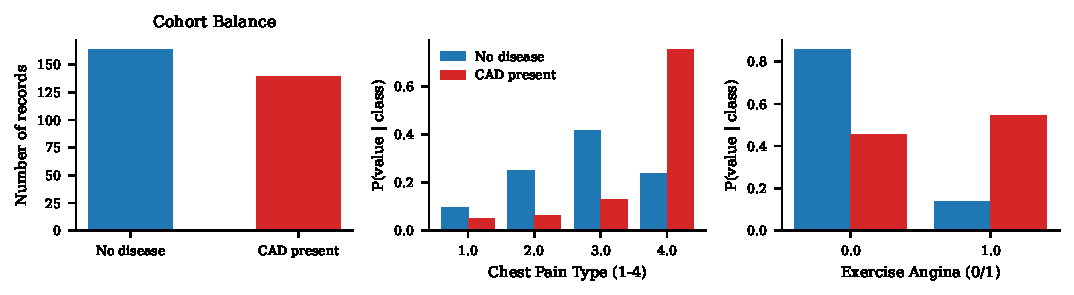
\includegraphics[width=\columnwidth]{f2}
\caption{Class counts and the within-class distributions of chest-pain type (\texttt{cp}) and exercise-induced angina (\texttt{exang}). The CAD group contains more asymptomatic chest-pain cases ($\texttt{cp}=4$) and more exercise-provoked angina.}
\label{fig:balance}
\end{figure}

Figure~\ref{fig:balance} shows the class counts and the observed symptom-category distributions in the cohort. The plotted proportions provide context for the categorical likelihoods used by Mixed NB.

\section{Mathematical Foundations}

\subsection{Bayesian Decision Theory and Conditional Independence}
Write the observed predictors as $\mathbf{x}=(x_1,\ldots,x_d)^\top$, and let $C\in\{0,1\}$ indicate disease status. Bayes' rule expresses the class posterior as
\begin{equation}
P(C=c\mid\mathbf{x})
=\frac{P(C=c)\,P(\mathbf{x}\mid C=c)}
{\sum_{k\in\{0,1\}} P(C=k)\,P(\mathbf{x}\mid C=k)}.
\end{equation}
The prior $P(C=c)$ is the class frequency before considering a patient's measurements. The likelihood $P(\mathbf{x}\mid C=c)$ describes how compatible those measurements are with class $c$, and the denominator normalizes the two class scores into probabilities. The Naive Bayes approximation treats predictors as independent once the class is known. In practical terms, each feature contributes its own class-specific likelihood. This makes the calculation manageable, though it cannot represent all relationships among clinical measurements. Under this assumption,
\begin{equation}
P(\mathbf{x}\mid C=c)=\prod_{j=1}^{d} P(x_j\mid C=c).
\end{equation}
Multiplying many small likelihoods can underflow in floating-point arithmetic. The class score is therefore computed as a sum of log-likelihoods:
\begin{equation}
\begin{aligned}
\log S(c\mid\mathbf{x})
&=\log P(C=c)\\
&\quad+\sum_{j\in\mathrm{NUM}}\log f_j(x_j\mid C=c)\\
&\quad+\sum_{j\in\mathrm{CAT}}\log P(x_j\mid C=c),
\end{aligned}
\end{equation}
Here, $\mathrm{NUM}=\{\texttt{age},\texttt{trestbps},\texttt{chol},\texttt{thalach}\}$ denotes the measurements and $\mathrm{CAT}=\{\text{cp},\text{exang}\}$ the categorical variables. A record is assigned to the positive class when the log-score difference reaches the selected threshold:
\begin{equation}
\hat{y}=
\begin{cases}
1, & \log S(1\mid\mathbf{x})-\log S(0\mid\mathbf{x})\ge\tau,\\
0, & \text{otherwise,}
\end{cases}
\end{equation}
The operating threshold is $\theta\in(0,1)$, with $\tau=\log\bigl(\theta/(1-\theta)\bigr)$. The default is $\theta=0.5$, corresponding to $\tau=0$.

The quantity $S(c\mid\mathbf{x})$ is an unnormalized class score, not itself a probability. Its log-score difference is the log posterior odds under the fitted model because the common normalizing denominator cancels between the two classes. A threshold of $0.5$ therefore assigns the record to the class with the larger score. Choosing a lower threshold changes the decision rule while leaving the fitted likelihoods unchanged; the resulting increase in sensitivity can be accompanied by a decrease in specificity, as examined in the threshold sweep.

\subsection{Continuous Features: Gaussian Likelihood}
For each numerical variable $x_j\in\mathrm{NUM}$, the class-conditional density is Gaussian:
\begin{equation}
f_j(x_j\mid C=c)
=\frac{1}{\sqrt{2\pi\sigma_{jc}^{2}}}
\exp\Bigl(-\frac{(x_j-\mu_{jc})^{2}}{2\sigma_{jc}^{2}}\Bigr).
\end{equation}
For a continuous measurement, $f_j(x_j\mid C=c)$ is a density rather than the probability of observing the exact value $x_j$. Probabilities correspond to areas under the density curve.
For class $c$, let $I_c$ index its $N_c$ training observations. The fitted mean and variance are
\begin{align}
\mu_{jc}&=\frac{1}{N_c}\sum_{i\in I_c}x_{ij},\\
\sigma_{jc}^{2}&=\max\Bigl(\frac{1}{N_c}\sum_{i\in I_c}(x_{ij}-\mu_{jc})^{2},\,\varepsilon_{\mathrm{floor}}\Bigr),
\end{align}
These are maximum-likelihood estimates, so the variance denominator is $N_c$ (equivalently, $\mathrm{ddof}=0$), rather than $N_c-1$ as in the unbiased sample variance. To avoid a singular density, estimates below $\varepsilon_{\mathrm{floor}}=10^{-6}$ are set to this floor.

\subsection{Categorical Features: Laplace Smoothing}
Each categorical predictor $x_j\in\mathrm{CAT}$ takes values in a finite set $\mathcal{K}_j$. Under a raw frequency estimate, a category absent from class $c$ in a training partition would receive probability zero and eliminate that class's full likelihood. Add-one smoothing avoids this outcome:
\begin{equation}
P(x_j=v\mid C=c)
=\frac{N_{jc}(v)+\alpha}{N_c+\alpha\,|\mathcal{K}_j|},
\end{equation}
The analysis sets $\alpha=1$, with $\mathcal{K}_{\text{cp}}=\{1,2,3,4\}$ and $\mathcal{K}_{\text{exang}}=\{0,1\}$; thus, $|\mathcal{K}_{\text{cp}}|=4$ and $|\mathcal{K}_{\text{exang}}|=2$. A level absent from a training partition consequently receives probability $\alpha/(N_c+\alpha|\mathcal{K}_j|)$, keeping the class score finite.

\subsection{Log-Sum-Exp Normalization}
To turn the two log-scores into a posterior without exponentiating unnecessarily large values, let $M=\max_c\log S(c\mid\mathbf{x})$ and subtract this common offset:
\begin{equation}
P(C=1\mid\mathbf{x})
=\frac{\mathrm{e}^{\log S(1\mid\mathbf{x})-M}}
{\mathrm{e}^{\log S(0\mid\mathbf{x})-M}+\mathrm{e}^{\log S(1\mid\mathbf{x})-M}}.
\end{equation}

\section{Methodology and Experimental Design}

\subsection{Leakage-Free Preprocessing}
Within each fold, the class priors $P(C=c)=N_c/N_{\mathrm{train}}$, Gaussian parameters $(\mu_{jc},\sigma_{jc}^{2})$, and categorical tables are estimated from training records only. The same separation is used for logistic regression: scaling and one-hot encoding are fitted on the training data and then applied to the test data, with missing dummy columns set to zero. The values $\alpha=1.0$ and $\varepsilon=10^{-6}$ were fixed before evaluation; test records were not used for tuning.

Each evaluation fold follows the same sequence: (1) separate training and test indices while preserving class proportions; (2) fit each model's preprocessing and parameters using the training portion; (3) predict positive-class probabilities for the held-out portion; and (4) calculate threshold-based scores, ROC-AUC, and Brier score from those predictions. The Gaussian NB ablation uses the same continuous variables and fold partitions as Mixed NB, while logistic regression uses all six selected fields after training-fold scaling and one-hot encoding. Sharing the fold partitions makes the model comparisons paired at the fold level, although repetition means those fold-level pairs are not mutually independent.

\subsection{Validation Protocols}
\begin{enumerate}
\item \textbf{Stratified holdout (80/20):} The split (seed $42$) assigns $242$ records to training ($131$ negative and $111$ positive) and $61$ to testing ($33$ negative and $28$ positive). Percentile confidence intervals at the $95\%$ level are calculated from $1{,}000$ bootstrap resamples.
\item \textbf{Repeated stratified $10 \times 5$-fold cross-validation:} Five-fold partitioning is repeated ten times, producing 50 folds (seed $1$). This serves as the main model comparison because a single test split provides limited evidence for a cohort of 303 patients.
\end{enumerate}
Stratification keeps the positive-to-negative ratio approximately stable in each partition. Each record consequently receives an out-of-fold prediction once per repeat, while each fold-level score is calculated only on records excluded from that fold's model fitting. The reported cross-validation mean is the arithmetic mean of the 50 fold scores; the reported SD describes their spread. Because repeated folds reuse observations, these summaries should not be interpreted as if they came from 50 independent cohorts.

\subsection{Baselines}
\begin{enumerate}
\item \textbf{Gaussian NB (numeric):} uses only the four continuous variables, providing a baseline for assessing the contribution of the symptom categories.
\item \textbf{$\ell_2$-regularized logistic regression:} takes standardized numerical measurements and one-hot indicators for chest pain and angina ($C=1.0$, 2000 iterations).
\item \textbf{Decision tree (fixed):} uses the four numerical features and one-hot indicators for both categorical features, with maximum depth 3 and minimum leaf size 5. These settings were fixed in advance; no hyperparameter search was performed.
\end{enumerate}

\subsection{Metrics}
Performance is summarized using accuracy, precision, recall (sensitivity), specificity, F1, ROC-AUC~\cite{fawcett2006}, and Brier score~\cite{brier1950}. Together, these measures describe both class decisions and probability quality. Because a false negative is especially consequential in a triage setting, recall is considered alongside the other classification measures; the Brier score and reliability plot assess agreement between predicted probabilities and outcomes. Fold-level AUCs for Mixed NB and logistic regression are compared with the Wilcoxon signed-rank test. The implementation uses scikit-learn~\cite{sklearn} and standard probability identities~\cite{bishop2006}.

For a binary confusion matrix with true positives (TP), false positives (FP), true negatives (TN), and false negatives (FN), the threshold-based measures are
\begin{align}
\mathrm{Accuracy}&=\frac{\mathrm{TP}+\mathrm{TN}}{\mathrm{TP}+\mathrm{FP}+\mathrm{TN}+\mathrm{FN}},\\
\mathrm{Precision}&=\frac{\mathrm{TP}}{\mathrm{TP}+\mathrm{FP}},\qquad
\mathrm{Recall}=\frac{\mathrm{TP}}{\mathrm{TP}+\mathrm{FN}},\\
\mathrm{Specificity}&=\frac{\mathrm{TN}}{\mathrm{TN}+\mathrm{FP}},\qquad
F_1=2\frac{\mathrm{Precision}\,\mathrm{Recall}}{\mathrm{Precision}+\mathrm{Recall}}.
\end{align}
ROC-AUC measures ranking over the range of possible thresholds, while the Brier score averages squared probability error, $N^{-1}\sum_i (p_i-y_i)^2$. Lower Brier scores indicate better overall probability accuracy, but the score alone does not isolate calibration from other aspects of predictive performance. All threshold-based measures use the default threshold of $0.5$, except for the explicitly reported threshold sweep.

The holdout confidence intervals are percentile intervals from resampling the 61 held-out cases with replacement. Repeated cross-validation provides fold-level variation across 50 test folds; because folds from repeated partitions are not independent samples, their standard deviations are descriptive and the paired Wilcoxon comparison is treated as exploratory rather than as a definitive significance test.

\section{Results}

\subsection{Assumption Diagnostics}
Shapiro--Wilk tests were applied separately to each continuous feature within each outcome class. At the $0.05$ level, the Gaussian assumption is rejected for resting blood pressure in CAD patients ($p=1.17\times10^{-4}$), cholesterol in controls ($p=2.88\times10^{-9}$), and maximum heart rate in controls ($p=5.43\times10^{-4}$). Cholesterol is positively skewed ($\mathrm{skew}=1.13$), and several recorded values exceed $400$\,mg/dl. The histograms and fitted class-conditional densities in Fig.~\ref{fig:gauss} illustrate how these departures vary across the four measurements.

The test results indicate that a Gaussian density is an approximation rather than a complete description of every class-conditional feature distribution. For age, the Shapiro--Wilk test also rejects normality in CAD records ($p=0.0023$); resting blood pressure in controls is rejected as well ($p=0.0116$). The test does not reject normality for cholesterol in CAD records ($p=0.403$) or maximum heart rate in CAD records ($p=0.352$). These diagnostics are applied to eight feature-by-class combinations at an unadjusted $0.05$ level and are interpreted descriptively; no multiplicity-adjusted family-wise inference is claimed. The model is retained for its transparent likelihood construction, while the deviations are noted as a limitation of the chosen family.

\begin{figure}[!t]
\centering
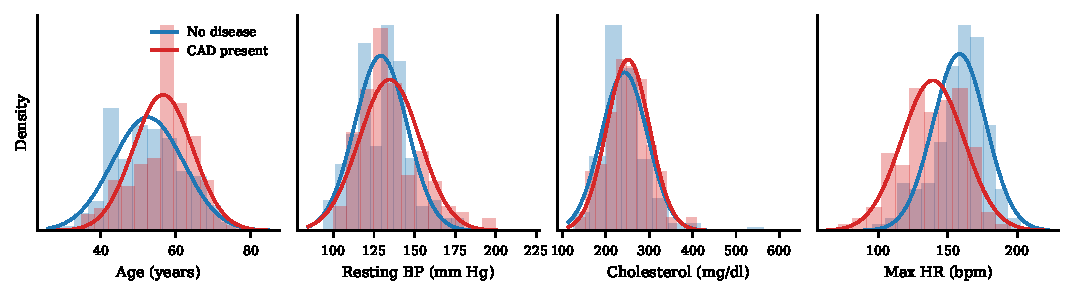
\includegraphics[width=\columnwidth]{f1}
\caption{Within-class histograms of the continuous predictors with fitted Gaussian curves. Maximum heart rate (\texttt{thalach}) separates the two classes most clearly.}
\label{fig:gauss}
\end{figure}

Pairwise Pearson coefficients are modest for most feature pairs, with $|r|<0.25$. The clearest departure occurs among controls: age and peak heart rate have $r=-0.523$ (Fig.~\ref{fig:corr}). This observed inverse association is a direct example of the conditional dependence that the model does not represent.

\begin{figure}[!t]
\centering
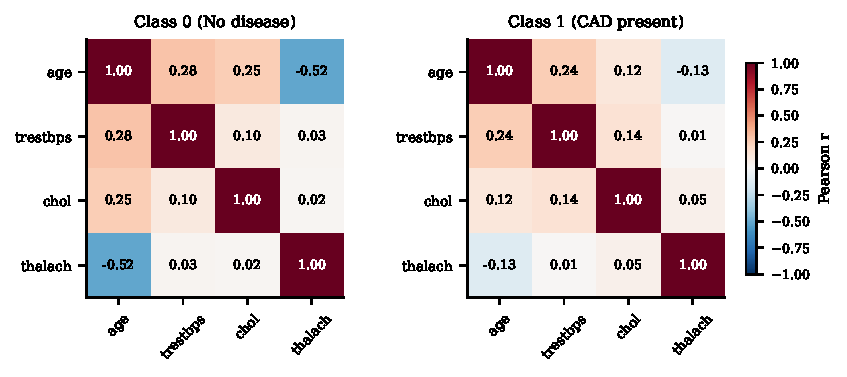
\includegraphics[width=\columnwidth]{f3}
\caption{Pearson correlation matrices calculated separately by class. Among controls, the largest association is between age and \texttt{thalach} ($r=-0.52$).}
\label{fig:corr}
\end{figure}

\subsection{Observed Feature Patterns}
The class summaries in Table~\ref{tab:cohort} show several differences that help describe the prediction task. Mean age is $4.04$ years higher in CAD-positive records, resting blood pressure is higher by $5.32$ mm\,Hg, and cholesterol is higher by $8.83$ mg/dl. Mean maximum heart rate is lower by $19.12$ beats/min in the CAD-positive group. These are marginal group contrasts: each is calculated without adjusting for the other predictors and should not be interpreted as an isolated effect.

The categorical distributions are particularly uneven. Chest-pain type 4 (asymptomatic) occurs in $105/139=75.5\%$ of CAD-positive records and $39/164=23.8\%$ of controls. Exercise-induced angina occurs in $76/139=54.7\%$ of positive records and $23/164=14.0\%$ of controls. Such separation offers a plausible empirical explanation for why the categorical-feature model outperforms the numeric-only ablation in this dataset. It does not establish that a single category causes CAD, nor does the comparison isolate the effect of chest-pain type from that of exercise angina; both features enter the mixed model together.

\subsection{Predictive Performance and Ablation}
The repeated $10 \times 5$-fold cross-validation and holdout estimates appear in Table~\ref{tab:results}. Across the 50 cross-validation folds, Mixed NB averages $74.8\%\pm4.8\%$ accuracy and $0.831\pm0.045$ ROC-AUC. In the numeric-only ablation, mean AUC is lower by $0.099$ ($0.732\pm0.052$), accuracy is lower by $7.1$ percentage points ($67.7\%\pm5.0\%$), and sensitivity is lower by $10.7$ percentage points ($60.7\%\pm8.2\%$ versus $71.4\%\pm7.3\%$). These are descriptive differences across repeated folds, not an independent-sample significance test. They suggest that the two smoothed symptom variables improve performance in this cohort, though the design does not isolate each variable's contribution or establish that the gain will generalize to another population.

\begin{table*}[!t]
\centering
\caption{Performance estimates for the cohort ($N=303$) using $10 \times 5$-fold cross-validation and one stratified holdout test set ($N=61$). Cross-validation cells give mean $\pm$ SD; bootstrap $95\%$ intervals are shown for holdout accuracy and AUC.}
\label{tab:results}
\renewcommand{\arraystretch}{1.18}
\setlength{\tabcolsep}{3pt}
{\scriptsize
\resizebox{\textwidth}{!}{%
\begin{tabular}{@{}llccccccc@{}}
\toprule
Classifier & Protocol & Accuracy & Precision & Recall & Specificity & F1 & ROC-AUC & Brier score \\
\midrule
Mixed NB (proposed) & \shortstack{$10 \times 5$-fold\\cross-validation}
  & $0.748\pm0.048$ & $0.733\pm0.064$ & $0.714\pm0.073$ & $0.776\pm0.070$
  & $0.721\pm0.055$ & $0.831\pm0.045$ & $0.183\pm0.032$ \\
Gaussian NB (numeric) & \shortstack{$10 \times 5$-fold\\cross-validation}
  & $0.677\pm0.050$ & $0.663\pm0.065$ & $0.607\pm0.082$ & $0.736\pm0.069$
  & $0.631\pm0.063$ & $0.732\pm0.052$ & $0.218\pm0.027$ \\
Logistic regression & \shortstack{$10 \times 5$-fold\\cross-validation}
  & $0.751\pm0.050$ & $0.743\pm0.072$ & $0.707\pm0.077$ & $0.788\pm0.073$
  & $0.722\pm0.058$ & $0.830\pm0.049$ & $0.168\pm0.026$ \\
Decision tree (fixed) & \shortstack{$10 \times 5$-fold\\cross-validation}
  & $0.713\pm0.049$ & $0.720\pm0.095$ & $0.649\pm0.124$ & $0.767\pm0.118$
  & $0.670\pm0.069$ & $0.808\pm0.050$ & $0.180\pm0.028$ \\
\midrule
Mixed NB (proposed) & Holdout
  & $0.803$ [$0.705$, $0.902$] & $0.767$ & $0.821$ & $0.788$
  & $0.793$ & $0.891$ [$0.803$, $0.960$] & $0.142$ \\
Gaussian NB (numeric) & Holdout
  & $0.721$ [$0.607$, $0.820$] & $0.720$ & $0.643$ & $0.788$
  & $0.679$ & $0.765$ [$0.627$, $0.875$] & $0.202$ \\
Logistic regression & Holdout
  & $0.820$ [$0.721$, $0.902$] & $0.815$ & $0.786$ & $0.848$
  & $0.800$ & $0.898$ [$0.814$, $0.966$] & $0.126$ \\
Decision tree (fixed) & Holdout
  & $0.754$ [$0.656$, $0.852$] & $0.810$ & $0.607$ & $0.879$ & $0.694$
  & $0.860$ [$0.759$, $0.939$] & $0.146$ \\
\bottomrule
\end{tabular}}}
\end{table*}

The paired fold comparison gives an average AUC difference of $+0.0011$ (fold-to-fold SD $0.0188$) for Mixed NB relative to logistic regression; the exploratory Wilcoxon result is $p=0.652$. This result does not provide evidence of a clear AUC difference, but it should not be read as proof of equivalence because the repeated folds are dependent and no equivalence margin was specified. Mean recall is $71.4\%$ for Mixed NB and $70.7\%$ for logistic regression; specificity is $77.6\%$ and $78.8\%$, respectively. The fixed decision tree has lower cross-validation recall ($64.9\%$) and F1 ($0.670$) than either model, though its results are descriptive and depend on the prespecified tree settings. Figure~\ref{fig:cvbars} displays the mean metrics across the folds, with one standard deviation shown for each estimate.

Across folds, logistic regression has slightly higher mean precision ($74.3\%$ versus $73.3\%$) and specificity ($78.8\%$ versus $77.6\%$), while Mixed NB has slightly higher recall ($71.4\%$ versus $70.7\%$). Their mean F1 values are nearly identical ($0.721$ and $0.722$). The numeric-only Gaussian model is lower on accuracy, precision, recall, F1, and AUC in these runs, while its specificity is also below the other two models. These measures give a fuller comparison than accuracy alone, particularly because the dataset has more controls than CAD-positive records.

\begin{figure}[!t]
\centering
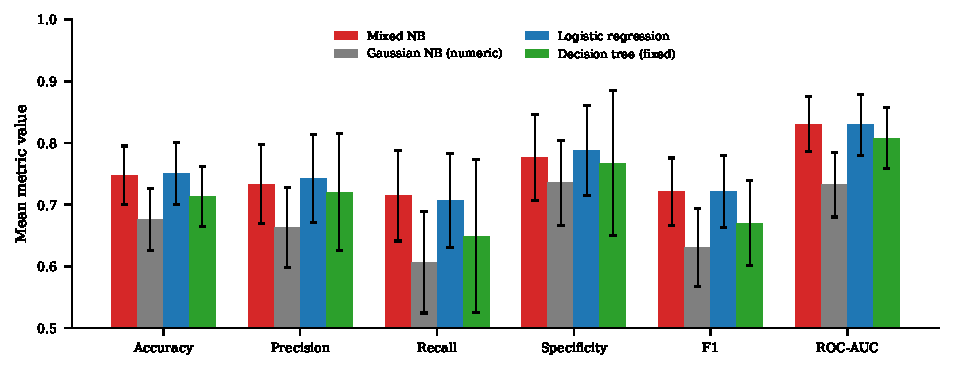
\includegraphics[width=\columnwidth]{f5}
\caption{Average values across the 50 validation folds; error bars show one standard deviation. Mixed NB and logistic regression perform similarly, while the numeric-only Gaussian model performs worse.}
\label{fig:cvbars}
\end{figure}

\subsection{Holdout Classification}
The test partition contains $28$ CAD cases and $33$ controls. Mixed NB correctly identifies $23$ cases and $26$ controls (Fig.~\ref{fig:cm}); it misses five positive cases and produces seven false positives. These predictions correspond to $80.3\%$ accuracy [95\% CI: $70.5\%$--$90.2\%$], $82.1\%$ recall, $78.8\%$ specificity, and $0.891$ AUC [95\% CI: $0.803$--$0.960$]. Logistic regression gives $82.0\%$ accuracy, $78.6\%$ recall, and $0.898$ AUC, with six false negatives and five false positives. The overlapping bootstrap intervals and small test set do not support a strong ranking of the two models; these holdout estimates are best read as an additional, single-split check rather than a conclusive comparison.

The holdout ranking differs slightly from the cross-validation averages: logistic regression has higher holdout accuracy and AUC, whereas Mixed NB identifies one more CAD-positive case at the fixed threshold. A single split can vary with which records happen to be assigned to testing, and the intervals are wide. Taken together, the holdout and repeated-CV results support the narrower conclusion that the two models show similar discrimination on this sample, not that one is uniformly superior.

\begin{figure}[!t]
\centering
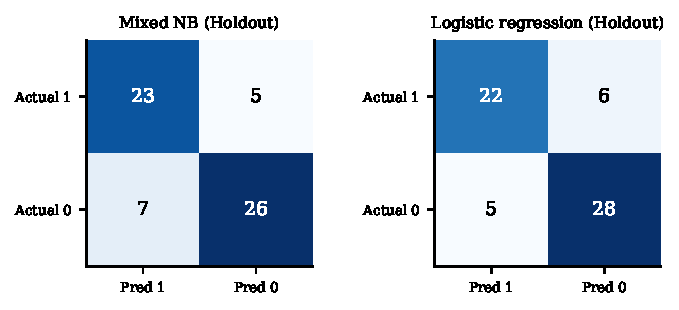
\includegraphics[width=\columnwidth]{f6}
\caption{Confusion matrices for the stratified test split ($N=61$), with CAD treated as the positive class. For Mixed NB, the counts are $23$ TP, $5$ FN, $7$ FP, and $26$ TN.}
\label{fig:cm}
\end{figure}

\subsection{Discrimination, Calibration, and Thresholds}
The pooled out-of-fold ROC curves in Fig.~\ref{fig:roc}(a) give AUCs of $0.830$ for Mixed NB, $0.731$ for Gaussian NB, $0.828$ for logistic regression, and $0.812$ for the fixed tree. These pooled AUCs are calculated from each record's out-of-fold probabilities averaged across the ten repeats; they differ slightly from the means of per-fold AUCs reported in Table~\ref{tab:results}, because AUC is computed after pooling in the figure and separately within each fold in the table. Probability calibration tells a different story. In Fig.~\ref{fig:roc}(b), logistic regression stays closer to the diagonal and has Brier score $0.168\pm0.026$; Mixed NB's reliability curve bends into an S shape, with Brier score $0.183\pm0.032$. Such a gap between ranking and probability accuracy is consistent with prior analyses of Naive Bayes~\cite{rish2001,niculescu2005}. When predictors share information, multiplying their likelihoods can make the posterior odds too extreme even when case ordering remains useful.

\begin{figure}[!t]
\centering
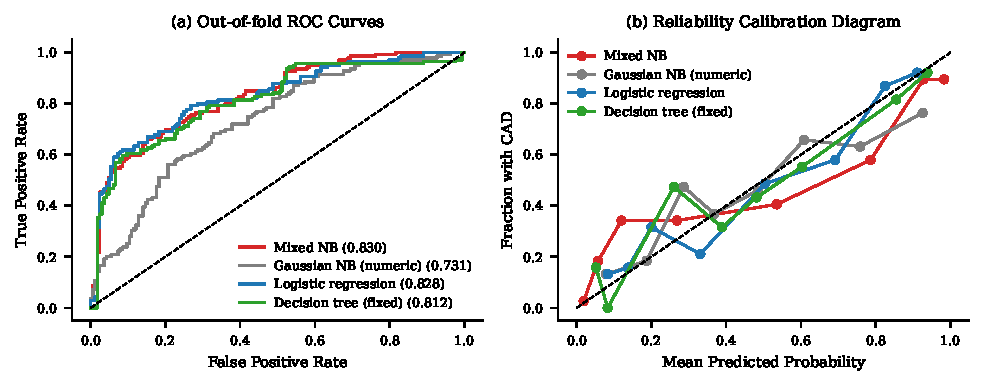
\includegraphics[width=\columnwidth]{f4}
\caption{(a) ROC curves and pooled AUCs from out-of-fold predictions averaged across ten repeats. (b) Reliability plots. Logistic regression has closer agreement between predicted and observed probabilities than Mixed NB.}
\label{fig:roc}
\end{figure}

The preferred operating threshold depends in part on how a missed ischemic case is weighed against an additional confirmatory test. Figure~\ref{fig:thr} illustrates this trade-off. The sweep uses Mixed NB out-of-fold probabilities for the 303 records, averaged over their ten held-out predictions; Table~\ref{tab:threshold} gives selected operating points. At $\theta=0.35$, recall is $77.0\%$ and specificity is $70.1\%$. This is an example from the dataset, not a clinically validated operating recommendation.

\begin{table}[!t]
\centering
\caption{Mixed NB threshold sweep on averaged out-of-fold predictions.}
\label{tab:threshold}
\setlength{\tabcolsep}{8pt}
\begin{tabular}{@{}ccc@{}}
\toprule
$\theta$ & Recall & Specificity \\
\midrule
0.30 & 0.770 & 0.659 \\
0.35 & 0.770 & 0.701 \\
0.40 & 0.763 & 0.707 \\
0.50 & 0.712 & 0.762 \\
\bottomrule
\end{tabular}
\end{table}

At the default threshold, the Mixed NB holdout confusion matrix contains five false negatives and seven false positives. The threshold sweep shows that a lower cutoff would classify more records as positive, reducing missed cases in this sample but increasing false alarms. Selecting between these operating points requires an explicit account of the consequences of each error, which this dataset and experiment do not supply. The sweep is therefore reported as a statistical illustration of the classifier's behavior, not as a recommendation for patient management.

\begin{figure}[!t]
\centering
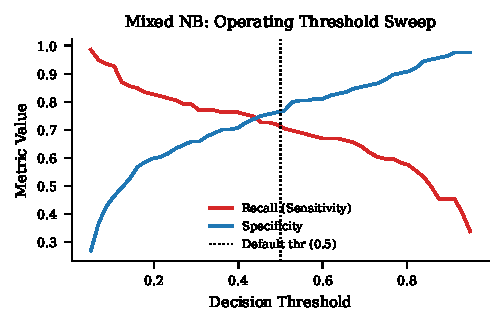
\includegraphics[width=\columnwidth]{f7}
\caption{Sensitivity and specificity of Mixed NB across operating thresholds. Reducing the threshold below $0.5$ increases sensitivity and decreases specificity.}
\label{fig:thr}
\end{figure}

\section{Discussion}
Adding chest-pain type and exercise-induced angina raises mean AUC by $0.099$ in this experiment. The class proportions help interpret this result: $75.5\%$ of CAD records are asymptomatic ($\texttt{cp}=4$), compared with $23.8\%$ of controls, and exercise-induced angina appears in $54.7\%$ of CAD cases versus $14.0\%$ of controls. These contrasts are descriptive associations in the Cleveland sample; they neither establish causation nor demonstrate that each feature independently accounts for the performance gain. Add-one smoothing handles levels that may be absent from a training fold without introducing a tuned smoothing parameter on this small cohort.

The majority-class accuracy for this dataset is $164/303=54.1\%$. Mixed NB's cross-validation accuracy of $74.8\%$ is higher, but accuracy alone would conceal the clinically relevant error balance: at the default threshold, cross-validation recall is $71.4\%$ and specificity is $77.6\%$. On the single holdout, recall is somewhat higher ($82.1\%$), with five CAD cases missed. The difference between cross-validation and holdout estimates illustrates why one favorable split should not be treated as a stable estimate of future performance.

Age and peak heart rate are related in the control group ($r=-0.523$), so the conditional-independence assumption is not literally true for these data. Mixed NB nevertheless has an AUC close to that of regularized logistic regression in repeated cross-validation. This pattern is compatible with the zero-one loss analysis by Domingos and Pazzani~\cite{domingos1997}: exact independence is not required for useful classification. It does not show that dependence is harmless in general, and the observed correlation may still affect probability estimates or performance on other samples.

The calibration results call for caution when interpreting a predicted probability as a risk estimate. Because Naive Bayes multiplies feature likelihoods, correlated predictors can contribute overlapping evidence and pull posterior probabilities toward the extremes. This interpretation is compatible with the observed difference between AUC and Brier score: AUC summarizes ranking, whereas Brier score penalizes probability errors. Applications that rely on risk levels or unequal error costs would need calibration assessed on data separate from the model-fitting data, for example through Platt scaling or isotonic regression. Such calibration was not performed here, so no recalibrated performance is claimed.

\section{Limitations and Ethical Considerations}
\begin{enumerate}
\item \textbf{Historical single-site cohort.} All $303$ patients came from Cleveland Clinic in the late 1980s. Changes in clinical practice and measurement technology limit the relevance of direct extrapolation; contemporary external validation would be needed before any clinical interpretation.
\item \textbf{Loss from dichotomization.} Mapping $\texttt{num}\in\{1,2,3,4\}$ to one positive class removes information about anatomical severity, including single-vessel, triple-vessel, and left-main disease.
\item \textbf{Small predictor set.} The six selected indicators make the mixed-type model easier to study, but they do not represent all available clinical information. Other fields, including ST depression, fluoroscopic vessel counts, and thallium scintigraphy, were not evaluated; \texttt{ca} and \texttt{thal} also contain missing values.
\item \textbf{Repeated-fold dependence.} The 50 test folds arise from ten repeated partitions of the same 303 records and are not independent samples. Fold means and standard deviations are useful summaries, but the paired Wilcoxon $p$-value is exploratory and should not be interpreted as a definitive population-level test.
\item \textbf{Single feature set and threshold.} The six predictors and default $0.5$ threshold were specified for this project; the results do not establish that these are optimal. The threshold sweep is descriptive and does not incorporate clinical utilities or decision costs.
\item \textbf{No clinical deployment claim.} This is an engineering and computational-statistics analysis. These models have not been tested prospectively and should not be used for autonomous triage or treatment.
\end{enumerate}

\section{Conclusion}
This study evaluated a mixed Gaussian-categorical Naive Bayes classifier on the Cleveland UCI cohort after establishing the target coding and keeping test data out of model fitting. Adding the smoothed symptom variables increased the $10 \times 5$-fold cross-validation AUC by $0.099$ relative to the continuous-only version, bringing it to $0.831$, close to logistic regression's $0.830$. The model ranked cases comparably despite departures from normality and conditional independence, while its probabilities were less well calibrated. Further work could test kernel density estimates, Bayesian networks that represent feature dependence, and post-hoc probability calibration.

\section*{Reproducibility Statement}
The analyses were run in Python 3.10 using NumPy, pandas, SciPy, scikit-learn, and Matplotlib. Random seeds were $42$ for the holdout split, $1$ for repeated CV, and $0$ for bootstrap resampling. The fixed parameters were $\alpha=1.0$, $\varepsilon=10^{-6}$, $\theta=0.5$, and, for the decision tree, maximum depth 3 and minimum leaf size 5. From the project directory, run \texttt{python experiments.py}; this reads \texttt{heart\_cleveland\_clean.csv} and regenerates \texttt{results.json} and the figures in \texttt{figs/}. The LaTeX report can be compiled with \texttt{tectonic paper.tex} (or an IEEE-compatible LaTeX installation). The accompanying code, cleaned dataset, results file, and generated figures are distributed with the project. Package installation and run steps are also listed in the project README.

\section*{AI Assistance Disclosure}
Generative AI tools were used as learning and editorial assistants to explain statistical concepts, revise manuscript wording and organization, review consistency between the report and project code, and suggest citation checks. The reported numerical results were generated by the documented Python pipeline; AI suggestions were not treated as evidence or as a substitute for cited sources. The author is responsible for verifying the data, code, calculations, references, and interpretations, and for understanding and explaining the work.

\begin{thebibliography}{99}

\bibitem{uci}
A.~Janosi, W.~Steinbrunn, M.~Pfisterer, and R.~Detrano,
``Heart Disease,''
UCI Machine Learning Repository, 1989.
[Online]. Available: \url{https://doi.org/10.24432/C52P4X}

\bibitem{who2025}
World Health Organization,
``Leading causes of death,''
[Online]. Available: \url{https://www.who.int/data/gho/data/themes/mortality-and-global-health-estimates/ghe-leading-causes-of-death}. Accessed: Oct. 22, 2026.

\bibitem{ahaCath}
American Heart Association,
``Cardiac catheterization,''
[Online]. Available: \url{https://www.heart.org/en/health-topics/heart-attack/diagnosing-a-heart-attack/cardiac-catheterization}. Accessed: Oct. 22, 2026.

\bibitem{detrano1989}
R.~Detrano, A.~Janosi, W.~Steinbrunn, M.~Pfisterer, J.~Schmid, S.~Sandhu, K.~Guppy, S.~Lee, and V.~Froelicher,
``International application of a new probability algorithm for the diagnosis of coronary artery disease,''
\textit{Amer.\ J.\ Cardiol.}, vol.~64, no.~5, pp.~304--310, 1989.

\bibitem{domingos1997}
P.~Domingos and M.~Pazzani,
``On the optimality of the simple Bayesian classifier under zero-one loss,''
\textit{Mach.\ Learn.}, vol.~29, no.~2, pp.~103--130, 1997.

\bibitem{rish2001}
I.~Rish,
``An empirical study of the naive Bayes classifier,''
in \textit{Proc.\ IJCAI Workshop Empirical Methods in AI}, Seattle, WA, USA, 2001, pp.~41--46.

\bibitem{sklearn}
F.~Pedregosa \textit{et al.},
``Scikit-learn: Machine learning in Python,''
\textit{J.\ Mach.\ Learn.\ Res.}, vol.~12, pp.~2825--2830, 2011.

\bibitem{fawcett2006}
T.~Fawcett,
``An introduction to ROC analysis,''
\textit{Pattern Recognit.\ Lett.}, vol.~27, no.~8, pp.~861--874, 2006.

\bibitem{brier1950}
G.~W.~Brier,
``Verification of forecasts expressed in terms of probability,''
\textit{Mon.\ Wea.\ Rev.}, vol.~78, no.~1, pp.~1--3, 1950.

\bibitem{niculescu2005}
A.~Niculescu-Mizil and R.~Caruana,
``Predicting good probabilities with supervised learning,''
in \textit{Proc.\ 22nd Int.\ Conf.\ Mach.\ Learn.\ (ICML)}, Bonn, Germany, 2005, pp.~625--632.

\bibitem{aha1988}
D.~W.~Aha,
``Heart Disease Databases Documentation,''
Dept.\ Inf.\ Comput.\ Sci., Univ.\ California, Irvine, Tech.\ Rep., Jul.\ 1988.

\bibitem{bishop2006}
C.~M.~Bishop,
\textit{Pattern Recognition and Machine Learning}.
New York, NY, USA: Springer, 2006.

\bibitem{khanna2015}
D.~Khanna, R.~Sahu, V.~Baths, and B.~Deshpande,
``Comparative study of classification techniques (SVM, logistic regression and neural networks) to predict the prevalence of heart disease,''
\textit{Int. J. Mach. Learn. Comput.}, vol.~5, no.~5, pp.~414--419, 2015, doi: 10.7763/IJMLC.2015.V5.544.

\bibitem{amin2019}
M.~S. Amin, Y.~K. Chiam, and K.~D. Varathan,
``Identification of significant features and data mining techniques in predicting heart disease,''
\textit{Telematics Inform.}, vol.~36, pp.~82--93, 2019, doi: 10.1016/j.tele.2018.11.007.

\bibitem{akella2021}
A.~Akella and S.~Akella,
``Machine learning algorithms for predicting coronary artery disease: Efforts toward an open source solution,''
\textit{Future Sci. OA}, vol.~7, no.~6, Art. no.~FSO698, 2021, doi: 10.2144/fsoa-2020-0206.

\bibitem{meidina2023}
A.~Meidina and Z.~Abidin,
``Diagnosis of heart disease using optimized Naive Bayes algorithm with particle swarm optimization and gain ratio,''
\textit{Recursive J. Inform.}, vol.~1, no.~2, pp.~47--54, 2023, doi: 10.15294/rji.v1i2.67278.

\end{thebibliography}

\end{document}
